\section{Analysis of Perceived Randomness}\label{section:analysis_of_perceived_randomness}
As mentioned in Subsection~\ref{subsection:data_analysis}, the analysis of this study's findings is performed using two methods: chi-square goodness-of-fit, and by comparing the differences in the cumulative loss of the Learner $L$ and each Expert $\mathcal{E}_i \in \{\mathcal{E}_1,\ldots, \mathcal{E}_N\}$. With these methods, this Chapter delves into the results to provide evidence for the hypothesised question ``Are humans good randomisers?''

\subsection{Chi-Square Goodness-of-Fit}\label{subsection:chi-square_goodness-of-fit}
We begin with the Chi-Squared ($\chi^2$) Goodness-of-Fit, a statistical method for determining if observed results are similar to what is expected from the null hypothesis\textemdash{}that humans are good randomisers.

\subsubsection{Distribution of the Number of Heads}
Figure~\ref{distribution_of_the_number_of_heads} shows that the distribution produced by the subjects is qualitatively similar to the theoretical distribution in that it is bell-shaped, however the results of $\chi^2(10, N=175) = 155.14, p=3.26\mathrm{e}{-28} < 0.0001$ strongly indicate that the binomial distribution is not a good fit, with large discrepancies found at either extreme, and for sequences with $7+$ heads. As noted in~\cite{nickerson:2009}, ``in a randomly produced set of toss sequences, about 25\% of the sequences should have five heads and about 65\% should have four to six heads.'' In this study's sequences, 34\% had exactly five, and 73\% had four to six heads.

\begin{figure}[h]
    \centering
    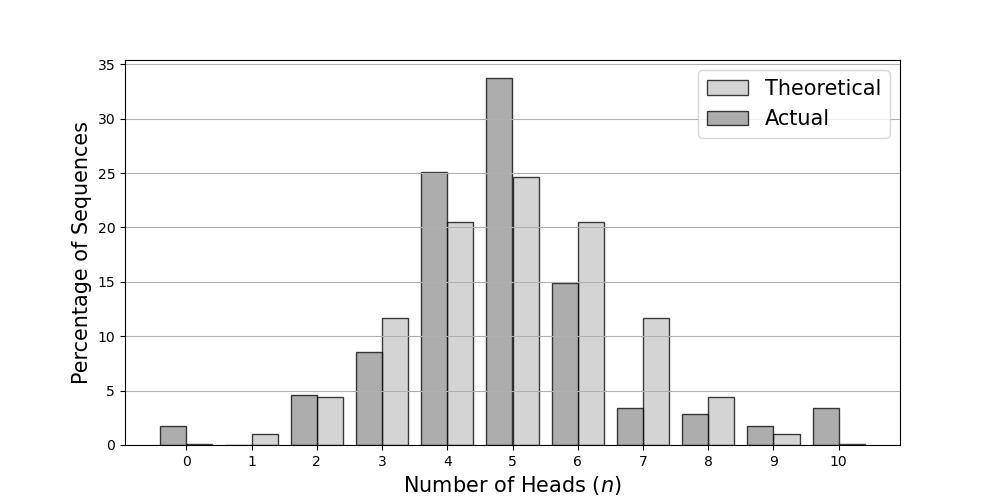
\includegraphics[width=0.9\textwidth]{images/combined_number_of_heads.jpg}
    \caption{Percentage of 10-Item Sequences with $n$ Heads, Compared to the Theoretical Distribution, $X \sim B(10, 0.5)$}\label{distribution_of_the_number_of_heads}
\end{figure}

Overall, these findings are more than significant enough to reject the null hypothesis and support the conclusion noted by Nickerson and Butler in that ``when trying to emulate a random generator of binary sequences, people are likely to produce a larger percentage of sequences that contain the two elements (e.g., heads and tails) in approximately equal proportions than is a random process.''~\cite{nickerson:2009}

\subsubsection{Distribution of the Number of Runs}
Unlike with the Distribution of the Number of Heads, the distribution produced by the subjects shown in Figure~\ref{distribution_of_the_number_of_runs} is both qualitatively and quantitatively different to what was expected, $\chi^2(9, N=175) = 908.46, p=9.29\mathrm{e}{-190} < 0.0001$. The produced distribution does not have a discernable bell shape, and instead, seems to steadily rise to $r = 8$ before significantly dropping off.


\begin{figure}[h]
    \centering
    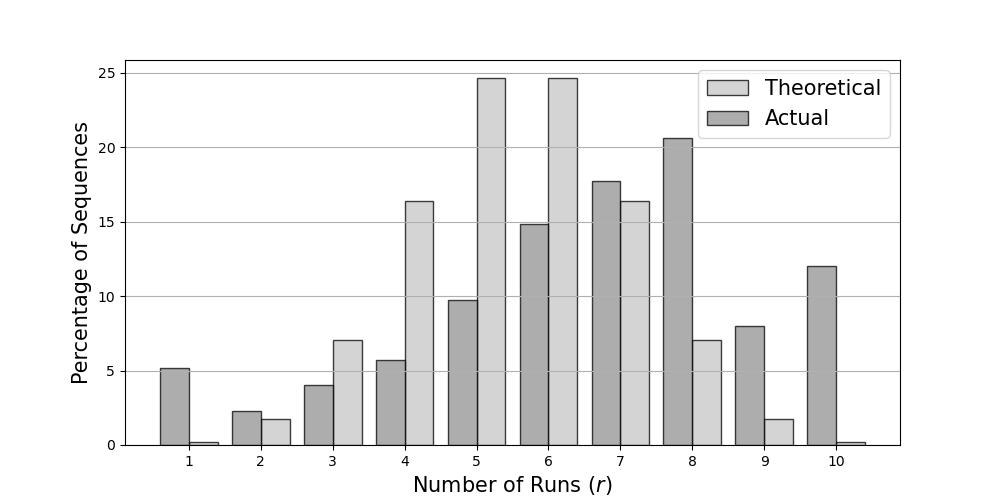
\includegraphics[width=0.9\textwidth]{images/combined_number_of_runs.jpg}
    \caption{Percentage of 10-Item Sequences with $r$ Runs, Compared to the Theoretical Distribution}\label{distribution_of_the_number_of_runs}
\end{figure}

Despite looking different to that produced by Nickerson and Butler, this data still supports their conclusion that ``people are likely to fail when trying to emulate a random process \textendash{} in this case by being less likely than a random process to produce sequences with an intermediate number of runs and more likely to produce sequences with close to the minimum or maximum number possible''~\cite{nickerson:2009}. The discrepancies that follow the peak at $r = 8$ also support Bar-Hillel and Wagenaar's conclusion that ``humans produce series with higher than expected alternation rates''~\cite{bar-hillel:1991}.

\subsubsection{Distribution of Run Lengths}
As previously defined, a \textit{run} is a consecutive sequence of the same outcome (either all heads or all tails), meaning that a run length of 1 occurs when only a single head or tail appears before the outcome changes. While the distribution produced by subjects appears qualitatively similar to the theoretical distribution in that the frequency of run lengths decreases exponentially, a significant percentage of runs more than expected had a length of 1, while all other run lengths were underrepresented in the data, $\chi^2(9, N=1,160) = 33.25, p=0.0001$.

\begin{figure}[h]
    \centering
    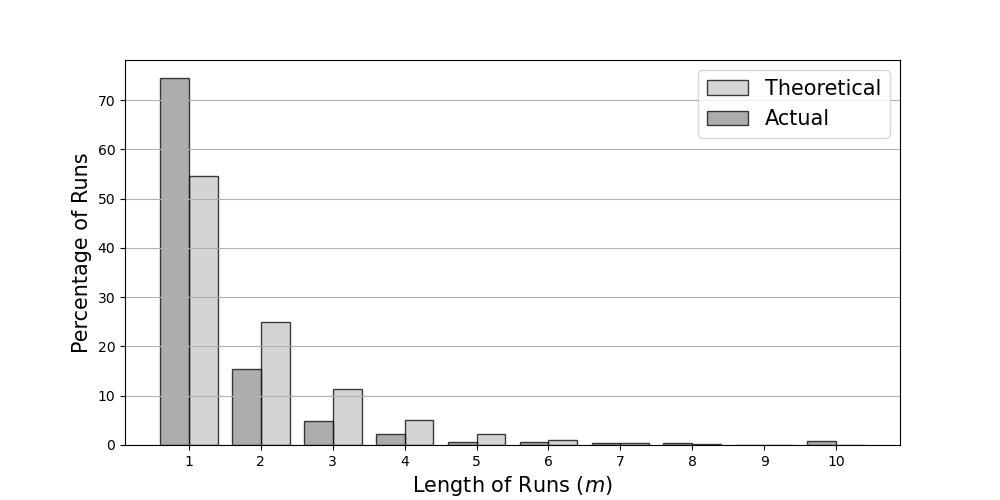
\includegraphics[width=0.9\textwidth]{images/combined_length_of_runs.jpg}
    \caption{Percentage of Runs with Length $m$, Compared to the Theoretical Distribution}
\end{figure}

Once again, this supports the conclusion drawn by~\cite{bar-hillel:1991} in that human-generated sequences favour alternation over continuation with 90\% of runs across all sequences being up to length $2$, and 97\% being up to length $4$.


\subsection{Regret Analysis}
Given the evidence shown in Subsection~\ref{subsection:chi-square_goodness-of-fit} supporting the conclusion that humans are not good randomisers, we now delve into an evaluation of the Aggregating Algorithm's performance at being able to predict the next bit of human-generated binary sequence.

As previously discussed, a Learner makes use of the predictions from several Experts to form their own about the next bit in a sequence entered by subjects after the fact (acting as Nature in this context). Continuing to assume the null hypothesis that humans are good randomisers, the Aggregating Algorithm should perform no better than randomly guessing the next bit of a sequence, i.e., having a 50\% success rate, however, the plot below shows that this is not the case for any of the subjects tested.

\begin{figure}[h]
    \centering
    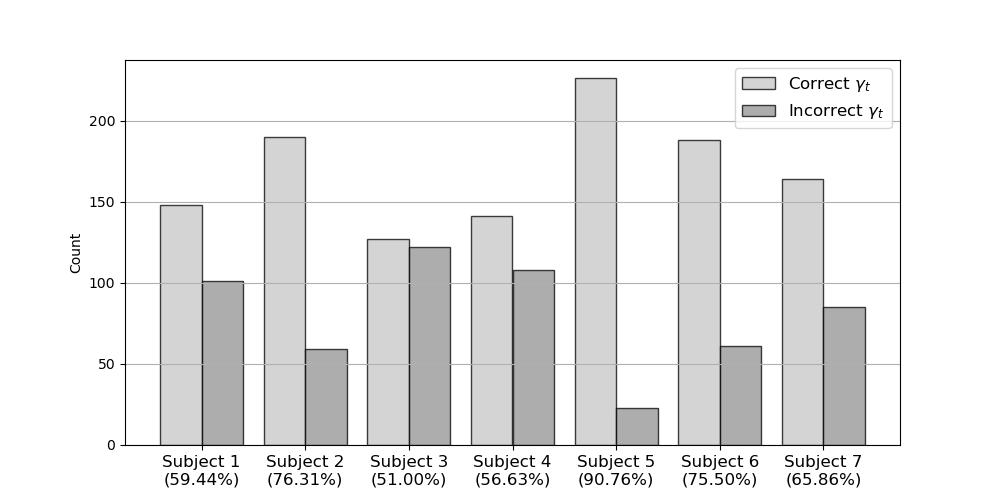
\includegraphics[width=0.9\textwidth]{images/prediction_results.jpg}
    \caption{Correct vs. Incorrect Predictions for Each Subject}\label{prediction_results}
\end{figure}

The performance of the Aggregating Algorithm exceeded that of random guessing across all subjects, although the improvement was only marginal for Subjects 3 and 4. On average, the Aggregating Algorithm achieved an accuracy of 69.19\%, reinforcing the notion that human-generated sequences exhibit predictable patterns, even when only considering prefixes up to length $4$.

\subsubsection{Statistical Significance of the Aggregating Algorithm's Performance}
To further investigate whether the Aggregating Algorithm performed significantly better than random guessing, a binomial significance test was conducted. The null hypothesis of the test presumes that the Aggregating Algorithm performs no better than random guessing, i.e., a success rate of 50\%\textemdash{}the probability of correctly predicting the next bit in the sequence by chance. The test was applied to the results from the seven subjects individually and in aggregate, using a significance level of $\alpha = 0.01$ to provide a comprehensive assessment of the algorithm's performance.

Individually, the results reveal that the Aggregating Algorithm performed significantly better than random guessing for five out of the seven subjects.  For Subjects 1, 2,5, 6, and 7, the p-values were well below the significance threshold, with Subjects 5 and 6 having exceptionally low p-values of $1.35\mathrm{e}{-48}$ and $1.40\mathrm{e}{-18}$ respectively. These values strongly indicate that the algorithm's predictions are extremely unlikely to be due to random chance. Additionally, Subjects 1, 2, and 7 had p-values of $1.30\mathrm{e}{-5}$, $1.53\mathrm{e}{-17}$, and $3.13\mathrm{e}{-7}$ respectively, further reinforcing the robustness of the algorithm's predictive performance. With a more lenient threshold of $\alpha = 0.05$, Subject 5's p-value of $0.00379$ would have also been significant. Conversely, Subjects 3 and 4 did not achieve statistically significant results, with p-values of $0.1875$ and $0.0379$ respectively, furthering the notion that individuals have different perceptions of randomness.

When analysing the results in aggregate, the algorithm's performance also remained significantly better than random guessing, with $P(X \geq 1206) < 0.00000001$. This indicates that observing 1,206 or more successes out of 1,743 trials by random chance alone is virtually impossible, ultimately emphasising the predictability of human-generated sequences and highlighting the strength of the Aggregating Algorithm in detecting the subconscious patterns of such sequences.

\subsubsection{Comparative Analysis of Cumulative Losses}
An examination of the difference in cumulative losses between individual Experts and the Learner across all time steps reveals patterns in the data. When the difference between an Expert's and the Learner's cumulative loss is positive (i.e., the line is above the x-axis), it indicates that the Expert's predictions are less accurate than those of the aggregated model. This implies that the Learner is more effectively aggregating the given predictions, and suggests that the subject is less predictable when inputting a certain prefix, as the relevant Expert's predictions are less accurate.

Conversely, when the difference is negative (i.e., the line is below the x-axis), the individual Expert's predictions outperform the Learner's aggregate. This scenario implies that the Learner's aggregation is less effective and that the subject's behaviour is more predictable for a given prefix as the relevant Expert's predictions are more accurate.

Reviewing the difference plots for all participants, shown below, it is noteworthy that only the Experts designed to detect a Markov Chain of Length 1\textemdash{}a first-order Markov Chain\textemdash{}displayed a difference greater than 2. This observation supports the existing literature: humans tend to avoid immediate repetition and exhibit subconscious longer-term patterns and dependencies that a first-order Markov Chain cannot capture. This is due to inherent memory constraints. For example, if a participant alternates between bits every two or three time steps, a first-order Markov Chain will be unable to detect the pattern and cause inaccurate predictions,

Furthermore, the results indicate that as a participant's sequences display more qualitative similarities to true randomness, the Aggregating Algorithm's predictive accuracy decreases. This is reflected in a greater proportion of lines closer to the x-axis, as well as alternating signs, signifying an increase in randomness due to the appearance of more inconsistent patterns.

\begin{figure}[hb]
    \centering
    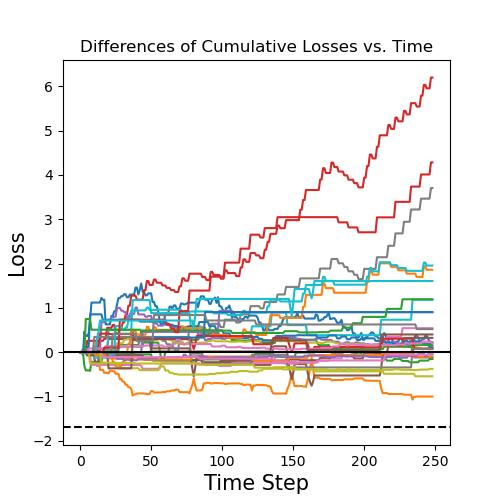
\includegraphics[width=0.625\textwidth]{images/AH_differences.jpg}
    \caption{Cumulative Loss Differences: Experts vs. Learner for Subject 1}
\end{figure}
\begin{figure}[ht]
    \centering
    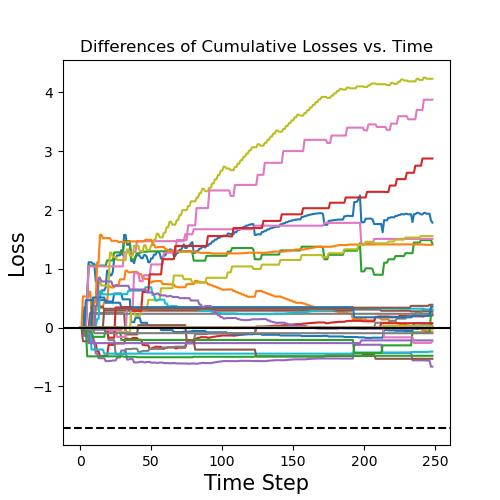
\includegraphics[width=0.625\textwidth]{images/EE_differences.jpg}
    \caption{Cumulative Loss Differences: Experts vs. Learner for Subject 2}
\end{figure}
\begin{figure}[h!]
    \centering
    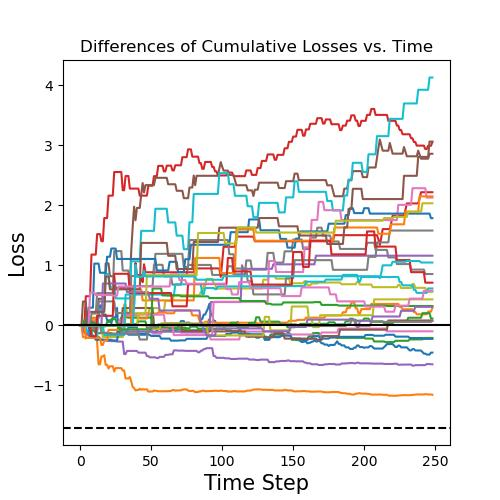
\includegraphics[width=0.625\textwidth]{images/HA_differences.jpg}
    \caption{Cumulative Loss Differences: Experts vs. Learner for Subject 3}
\end{figure}
\begin{figure}[ht]
    \centering
    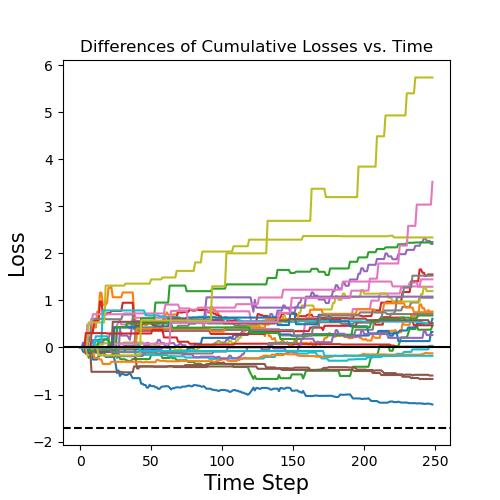
\includegraphics[width=0.625\textwidth]{images/ME_differences.jpg}
    \caption{Cumulative Loss Differences: Experts vs. Learner for Subject 4}
\end{figure}
\begin{figure}[h!]
    \centering
    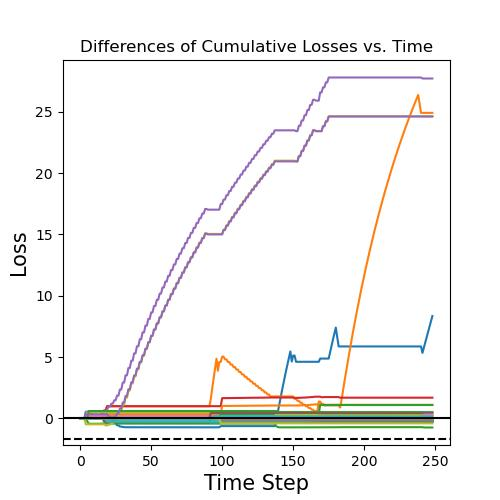
\includegraphics[width=0.625\textwidth]{images/NJ_differences.jpg}
    \caption{Cumulative Loss Differences: Experts vs. Learner for Subject 5}
\end{figure}
\begin{figure}[ht]
    \centering
    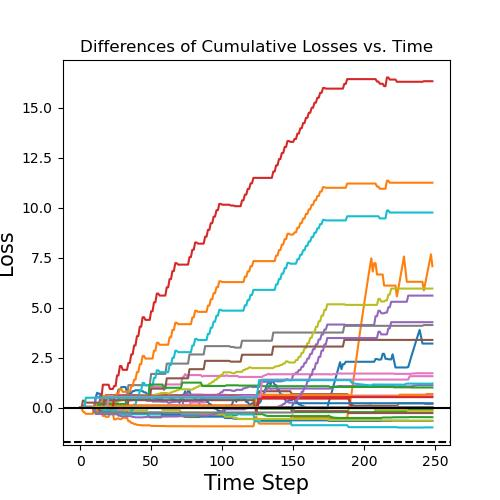
\includegraphics[width=0.625\textwidth]{images/RM_differences.jpg}
    \caption{Cumulative Loss Differences: Experts vs. Learner for Subject 6}
\end{figure}
\begin{figure}[h!]
    \centering
    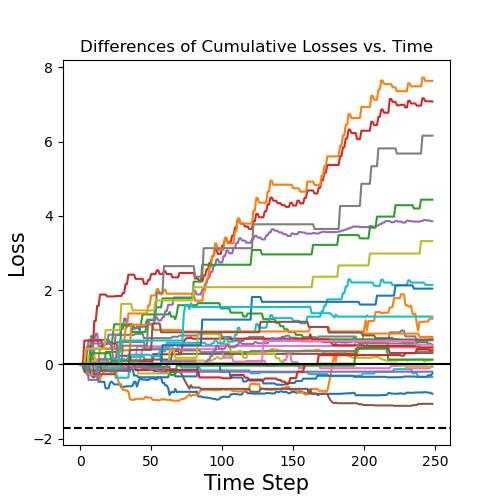
\includegraphics[width=0.625\textwidth]{images/RY_differences.jpg}
    \caption{Cumulative Loss Differences: Experts vs. Learner for Subject 7}
\end{figure}